%================================================
%	PACKAGES AND THEMES
%================================================
\documentclass[t,aspectratio=169,xcolor=dvipsnames]{beamer}

\usetheme{SimplePlusAIC}

% \usepackage{hyperref} % Beamer loads this automatically
\usepackage{graphicx} % Allows including images
\usepackage{booktabs} % Allows the use of \toprule, \midrule and  \bottomrule in tables
\usepackage{svg} % Allows using svg figures
\usepackage{tcolorbox} % For colored boxes
\usepackage{tikz}
\usepackage{makecell}
\newcommand*{\defeq}{\stackrel{\text{def}}{=}}
\usepackage{setspace}
\usepackage[T1]{fontenc}
\usepackage{helvet}
\usepackage{textgreek}
\usepackage{amsmath}
\usepackage{bm}
\usepackage{ragged2e}
\usepackage{xfrac}
% \usepackage[nice]{nicefrac}
\usepackage[loose]{units}
\usepackage{braket}
\usepackage{physics}
\usepackage{gensymb}
% \usepackage[cm]{sfmath}
\usepackage{verbatim}
\usepackage{fancyvrb}

%\setbeamertemplate{blocks}[rounded][shadow] % block options

\usepackage[svgnames,table]{xcolor}
\arrayrulecolor{black}
\setlength{\arrayrulewidth}{0.20mm}
\renewcommand{\arraystretch}{1.40}  % stretch tables row size

% Custom commands
\newcommand{\tem}[1]{\textbf{\textcolor{red}{#1}}}

%================================================
%	TITLE PAGE
%================================================
\title[Pengenalan OS]{Pengenalan Sistem Operasi}
\subtitle{Weeks 1: Konsep Dasar}

\author[lectura.id/os]{lectura.id/os}
\institute[ITERA]{Program Studi Teknik Informatika \\ Institut Teknologi Sumatera}

\date{\textcolor{nyublue}{2026}}

%================================================
%	BEGIN DOCUMENT 
%================================================
\begin{document}

%------------------------------------------------
%	TITLE SLIDE
%------------------------------------------------
\begin{frame}[plain]

    \titlepage
    
\end{frame}

%------------------------------------------------
%	OUTLINE SLIDE
%------------------------------------------------
\begin{frame}[plain]

    \frametitle{OUTLINE} 
    \framesubtitle{~}

    \begin{spacing}{1.2}
        \tableofcontents
    \end{spacing}
    
\end{frame}

%------------------------------------------------
%	LEARNING OUTCOMES
%------------------------------------------------
\begin{frame}[t]
    \frametitle{Capaian Pembelajaran (Learning Outcomes)}
    \framesubtitle{Apa yang akan kita pelajari hari ini/semester ini?}

    Setelah mengikuti mata kuliah/pertemuan ini, mahasiswa diharapkan mampu:
    \begin{itemize}
        \item \textbf{Memahami peran fundamental} Sistem Operasi sebagai manajer sumber daya (Resource Manager).
        \item \textbf{Menjelaskan konsep Virtualisasi} pada CPU dan Memori.
        \item \textbf{Mengidentifikasi tantangan} dalam Konkurensi dan menjaga Persistensi data.
        \item \textbf{Mengenal sejarah evolusi} Sistem Operasi dari masa ke masa.
    \end{itemize}
\end{frame}

\section{Pendahuluan}

%------------------------------------------------
\begin{frame}[plain]
    \begin{center}
        \vspace{3cm}
        \Huge\textbf{Pendahuluan}
    \end{center}
\end{frame}

%------------------------------------------------
\begin{frame}[t]
    \frametitle{Apa yang Sebenarnya Dilakukan Program?}
    \framesubtitle{Memahami Cara Kerja Dasar Komputer}
    
    \begin{alertblock}{Konsep Dasar}
        Program komputer itu sebenarnya sangat sederhana, dia hanya \tem{mengeksekusi instruksi} satu per satu.
    \end{alertblock}
    \vspace{0.3cm}
    
    \small
    Bayangkan sebuah program seperti resep masakan yang dijalankan langkah demi langkah oleh koki (prosesor).
    
    Prosesor melakukan siklus berulang yang disebut \tem{Von Neumann}:
    \begin{enumerate}
        \item \textbf{Fetch} (Ambil instruksi dari memori)
        \item \textbf{Decode} (Cari tahu apa arti instruksi itu)
        \item \textbf{Execute} (Jalankan perintahnya)
    \end{enumerate}
    
    Setelah selesai satu, dia pindah ke instruksi berikutnya. Begitu terus, jutaan bahkan miliaran kali per detik!
\end{frame}

%------------------------------------------------
\begin{frame}[plain]
    \vfill
    \centering
    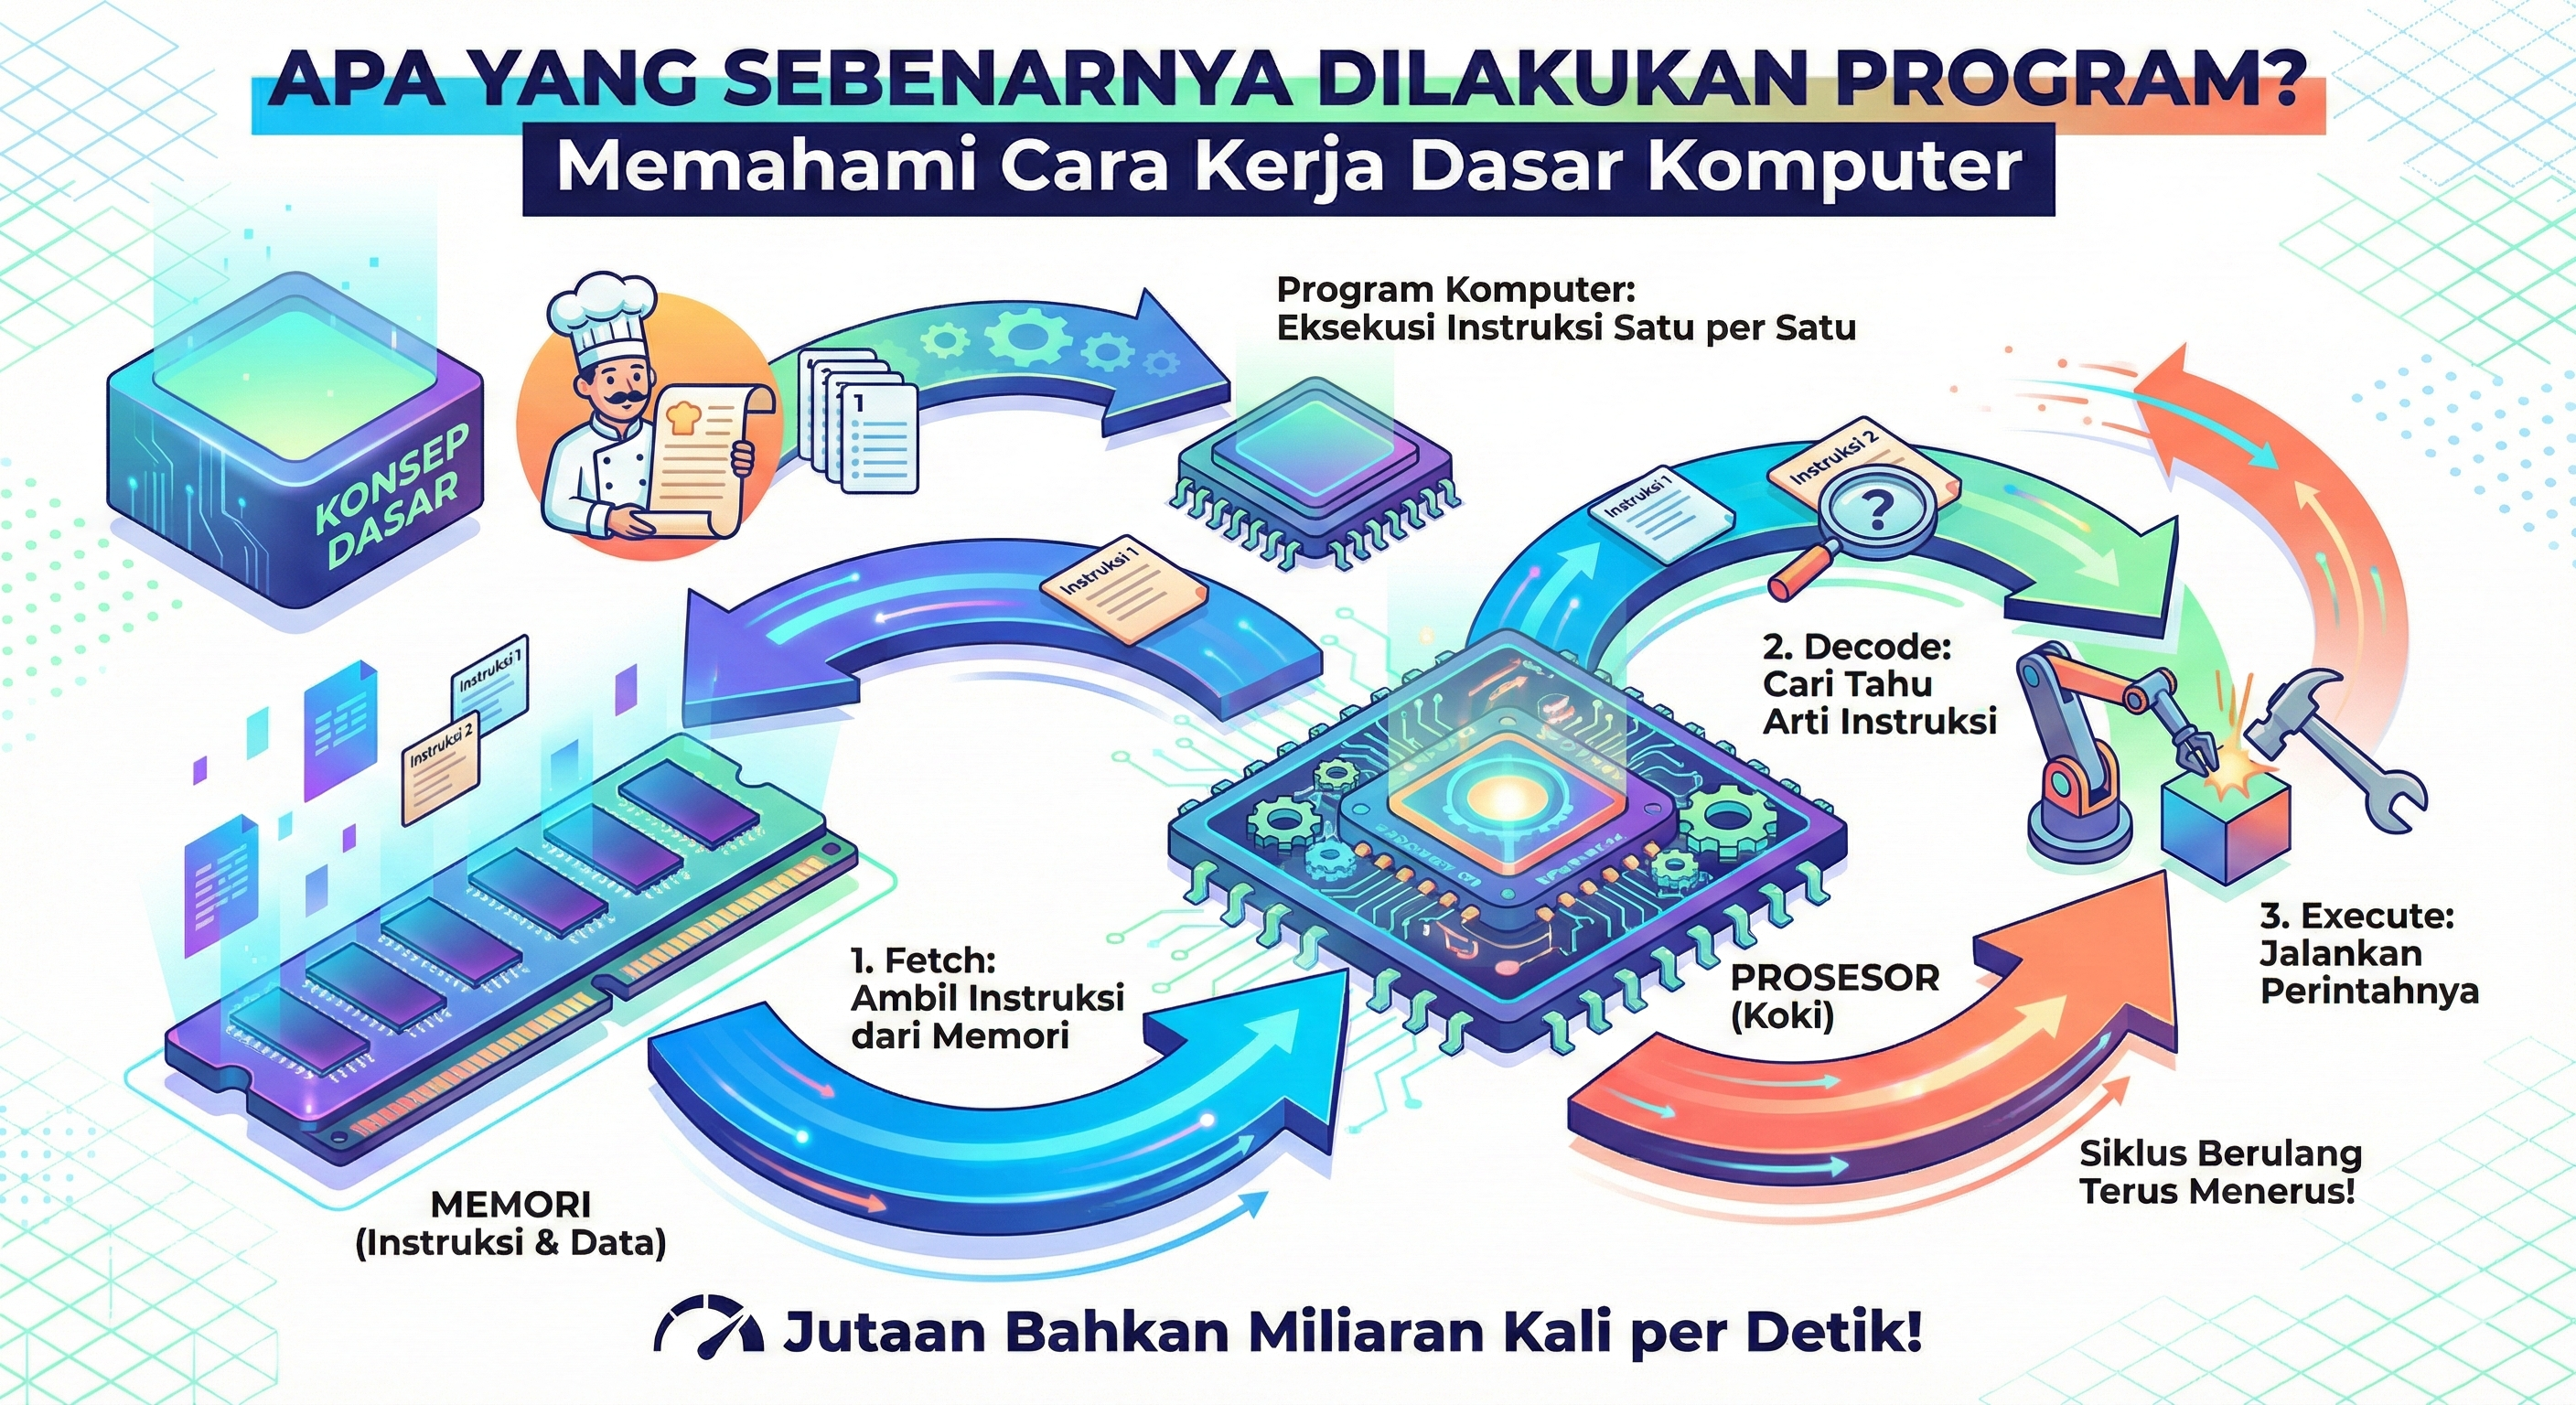
\includegraphics[width=0.93\paperwidth,keepaspectratio]{figures/1_program.png}
    \vfill
\end{frame}


%------------------------------------------------
\begin{frame}[t]
    \frametitle{Masalah Utama (The Crux)}
    \framesubtitle{Tantangan dalam Membangun Sistem Operasi}
    
    \begin{exampleblock}{Tantangan Kita}
        Bagaimana cara kita \tem{memvirtualisasi sumber daya} agar sistem mudah digunakan, efisien, dan aman?
    \end{exampleblock}
    \vspace{0.3cm}
    
    \small
    Kita ingin mengubah sumber daya fisik (seperti prosesor, memori, dan disk) menjadi bentuk virtual yang lebih hebat.
    
    \vspace{0.2cm}
    Mengapa?
    \begin{itemize}
        \item Agar banyak program bisa jalan bersamaan.
        \item Agar program tidak saling ganggu.
        \item Agar pengguna lebih mudah memakai komputer.
    \end{itemize}
\end{frame}

%------------------------------------------------
\begin{frame}[t]
    \frametitle{Apa itu Sistem Operasi?}
    \framesubtitle{Peran OS dalam Sistem Komputer}
    
    \begin{block}{Definisi Sederhana}
        Sistem Operasi (OS) adalah \tem{Manajer Sumber Daya} yang mengatur CPU, Memori, dan Disk komputer kita.
    \end{block}
    \vspace{0.3cm}
    
    \small
    OS menyediakan sekumpulan "tombol ajaib" (system calls) yang bisa dipanggil oleh program aplikasi.
    
    Sistem Operasi bertugas:
    \begin{enumerate}
        \item Memastikan sistem beroperasi dengan benar.
        \item Menjalankan program dengan efisien.
        \item Mengelola perangkat keras yang rumit sehingga programmer tidak perlu pusing.
    \end{enumerate}
\end{frame}

%------------------------------------------------
%	CLASS ACTIVITY 1
%------------------------------------------------
\begin{frame}[t]
    \frametitle{Aktivitas Kelas: Brainstorming}
    \framesubtitle{Diskusi Sederhana}

    \begin{alertblock}{Tantangan Dapur Restoran}
        Bayangkan sebuah dapur restoran yang hanya punya \textbf{1 Koki} (CPU) dan \textbf{1 Kompor} (Resource), tapi ada \textbf{3 Pesanan} (Process) yang datang bersamaan: Nasi Goreng, Sup Ayam, dan Telur Dadar.
    \end{alertblock}
    \vspace{0.3cm}

    \textbf{Diskusikan dengan teman sebelasmu (2-3 menit):}
    \begin{itemize}
        \item Bagaimana cara koki menangani ini agar semua pelanggan merasa dilayani dengan cepat?
        \item Apa yang terjadi jika koki hanya fokus menyelesaikan 1 pesanan sampai tuntas baru pindah ke pesanan lain?
    \end{itemize}
\end{frame}

\section{Virtualisasi}

%------------------------------------------------
\begin{frame}[plain]
    \begin{center}
        \vspace{3cm}
        \Huge\textbf{Virtualisasi}
    \end{center}
\end{frame}

%------------------------------------------------
\begin{frame}[t]
    \frametitle{Virtualisasi CPU}
    \framesubtitle{Membuat Satu CPU Terasa Seperti Banyak}
    
    \begin{block}{Ilusi Banyak CPU}
        OS mengubah satu CPU fisik menjadi seolah-olah ada \tem{banyak CPU virtual} yang tak terbatas.
    \end{block}
    \vspace{0.3cm}
    
    \small
    Bagaimana caranya? Dengan teknik \textit{Time Sharing}.
    
    OS menjalankan satu proses sebentar, lalu berhenti, menjalankan proses lain sebentar, dan seterusnya. Karena pergantian ini sangat cepat, kita merasa semua program berjalan bersamaan!
    
    \vspace{0.2cm}
    \textbf{Contoh:}
    \begin{itemize}
        \item Kamu bisa mendengarkan musik sambil mengetik tugas dan mengunduh file sekaligus.
        \item Padahal fisiknya, CPU melayani mereka bergantian satu per satu dengan sangat ngebut.
    \end{itemize}
\end{frame}

\begin{frame}[plain]
    \vfill
    \centering
    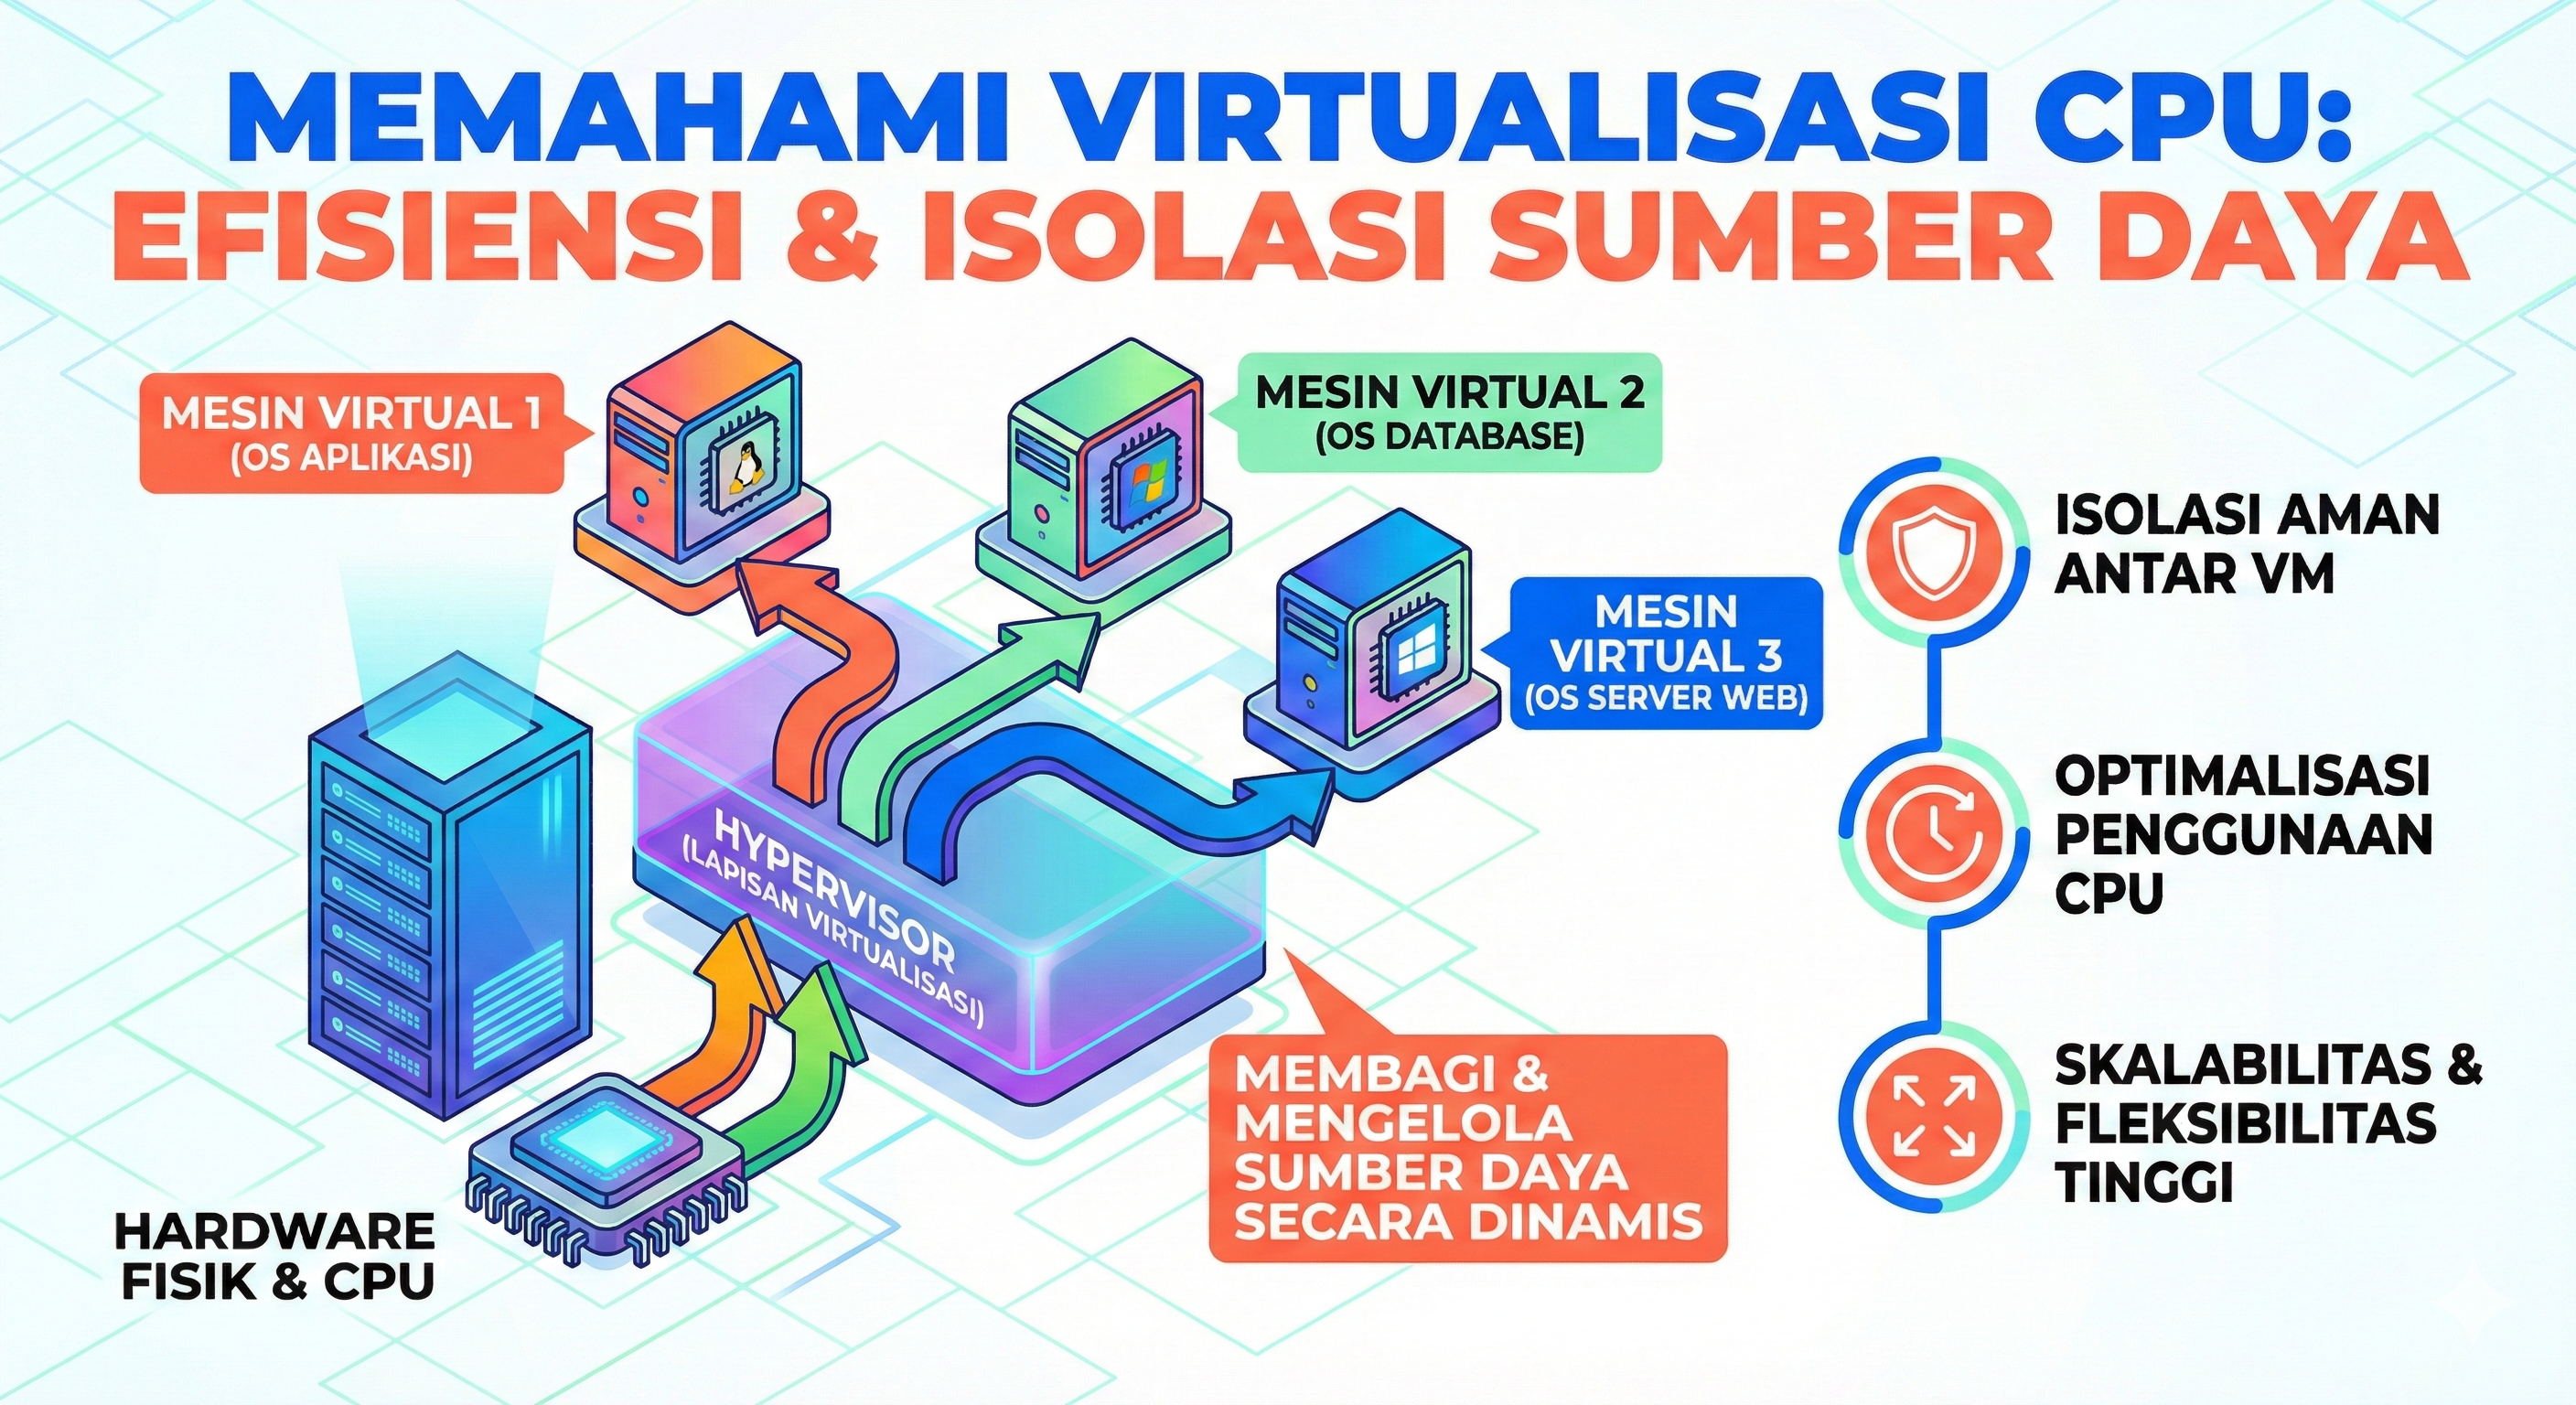
\includegraphics[width=0.93\paperwidth,keepaspectratio]{figures/1_virtualization.png}
    \vfill
\end{frame}

%------------------------------------------------
\begin{frame}[t]
    \frametitle{Virtualisasi Memori}
    \framesubtitle{Memberikan Ruang Privat untuk Setiap Program}
    
    \begin{alertblock}{Ruang Pribadi}
        Setiap program yang berjalan merasa memiliki \tem{memori sendiri} yang besar dan privat, padahal sebenarnya berbagi.
    \end{alertblock}
    \vspace{0.3cm}
    
    \small
    Ini disebut \textit{Ruang Alamat Virtual}.
    
    \begin{columns}[t]
        \column{0.5\textwidth}
           Apa untungnya?
           \begin{enumerate}
               \item \textbf{Aman}: Program A tidak bisa membaca atau mengacak-acak data milik Program B.
               \item \textbf{Mudah}: Programmer tidak perlu tahu di mana data sebenarnya disimpan secara fisik di RAM.
           \end{enumerate}
        \column{0.5\textwidth}
            OS secara diam-diam memetakan alamat virtual program ke alamat fisik yang sebenarnya di RAM komputer.
    \end{columns}
\end{frame}

\section{Konkurensi \& Persistensi}

%------------------------------------------------
\begin{frame}[plain]
    \begin{center}
        \vspace{3cm}
        \Huge\textbf{Konkurensi \& Persistensi}
    \end{center}
\end{frame}

%------------------------------------------------
\begin{frame}[t]
    \frametitle{Masalah Konkurensi}
    \framesubtitle{Tantangan Melakukan Banyak Hal Sekaligus}
    
    \begin{block}{Kerja Bareng Itu Susah}
        Masalah aneh dan rumit bisa muncul ketika kita mengerjakan \tem{banyak hal} sekaligus dalam satu program.
    \end{block}
    \vspace{0.1cm}
    
    \small
    Bayangkan dua orang mencoba mencatat skor di papan tulis yang sama secara bersamaan. Jika tidak hati-hati, catatannya bisa berantakan!
    
    \vspace{0.1cm}
    Contoh di Komputer:
    \scriptsize
    \begin{itemize}
        \item Program multi-thread punya variabel penghitung (counter).
        \item Thread 1 mau tambah 1.
        \item Thread 2 mau tambah 1.
        \item Jika mereka melakukannya persis bersamaan tanpa aturan, hasilnya bisa salah (bukan bertambah 2, tapi cuma 1).
    \end{itemize}
    OS harus menyediakan alat untuk menangani ini agar data tetap benar.
\end{frame}

%------------------------------------------------
\begin{frame}[t]
    \frametitle{Persistensi (Menyimpan Data)}
    \framesubtitle{Menjaga Data Agar Tidak Hilang}
    
    \begin{exampleblock}{Jangan Sampai Hilang}
        Memori (RAM) itu mudah lupa, jadi kita butuh \tem{penyimpanan permanen} seperti Hard Disk atau SSD.
    \end{exampleblock}
    \vspace{0.3cm}
    
    \small
    Data di RAM akan hilang kalau listrik mati atau komputer dimatikan (volatile).
    
    Bagaimana OS mengatasinya?
    \begin{enumerate}
        \item Mengelola perangkat penyimpanan (Disk/SSD).
        \item Menggunakan \textbf{File System} untuk mengatur data dalam bentuk file dan folder.
        \item Menggunakan teknik canggih (seperti \textit{journaling}) agar data tidak rusak kalau tiba-tiba komputer hang/mati saat menulis.
    \end{enumerate}
\end{frame}

\section{Desain \& Sejarah}

%------------------------------------------------
\begin{frame}[plain]
    \begin{center}
        \vspace{3cm}
        \Huge\textbf{Desain \& Sejarah}
    \end{center}
\end{frame}

%------------------------------------------------
\begin{frame}[t]
    \frametitle{Apa Tujuan Desain OS?}
    \framesubtitle{Kinerja, Perlindungan, dan Keandalan}
    
    \begin{block}{Tiga Pilar Utama}
        Sistem operasi dirancang untuk memberikan \tem{kinerja tinggi}, \tem{perlindungan}, dan \tem{keandalan}.
    \end{block}
    \vspace{0.3cm}
    
    \small
    Kita harus pintar memilih kompromi (\textit{trade-off}):
    
    \begin{columns}[t]
        \column{0.48\textwidth}
            \textbf{Abstraksi} \\
            Membuat sistem yang rumit jadi terasa sederhana digunakan.
            
            \vspace{0.2cm}
            \textbf{Kinerja (Performance)} \\
            Meminimalkan "overhead". Jangan sampai OS malah bikin komputer jadi lambat.
            
        \column{0.48\textwidth}
            \textbf{Perlindungan (Protection)} \\
            Isolasi program jahat atau error agar tidak merusak sistem (OS tidak boleh crash cuma karena satu aplikasi error).
    \end{columns}
\end{frame}

% (Redundant summary slide removed)

%------------------------------------------------
\begin{frame}[t]
    \frametitle{Sejarah OS: Era Awal (1950-an)}
    \framesubtitle{Manusia Sebagai Operator}
    
    \begin{columns}
        \column{0.6\textwidth}
        \begin{itemize}
            \item Belum ada Sistem Operasi yang canggih.
            \item Komputer adalah mesin raksasa (Mainframe).
            \item \textbf{Single User}: Satu orang menggunakan mesin pada satu waktu.
            \item Programmer berinteraksi langsung dengan hardware (plugboards, punch cards).
        \end{itemize}
        
        \vspace{0.2cm}
        \textbf{Masalah}: Waktu setup lama, CPU sering menganggur (\textit{idle}) menunggu manusia menyiapkan hal berikutnya.
    \end{columns}
\end{frame}

%------------------------------------------------
\begin{frame}[t]
    \frametitle{Sejarah OS: Era Batch \& Multiprogramming (1960-an)}
    \framesubtitle{Meningkatkan Utilitas CPU}
    
    \begin{block}{Batch Processing}
        Mengumpulkan pekerjaan (jobs) yang mirip dan menjalankannya secara berurutan untuk mengurangi waktu setup.
    \end{block}
    
    \begin{alertblock}{Multiprogramming}
        Lompatan besar! Memuat banyak program ke memori sekaligus.
        \begin{itemize}
            \item Saat Job A menunggu I/O (misal baca tape), CPU pindah ke Job B.
            \item \textbf{Tantangan Baru}: Perlindungan memori (agar Job A tidak merusak Job B) dan Concurrency.
        \end{itemize}
    \end{alertblock}
\end{frame}

%------------------------------------------------
\begin{frame}[t]
    \frametitle{Sejarah OS: Era Time-Sharing (1970-an)}
    \framesubtitle{Lahirnya Interaktivitas dan UNIX}
    
    \begin{itemize}
        \item \textbf{Time-Sharing}: CPU berpindah sangat cepat antar user. User merasa memiliki mesin sendiri (interaktif).
        \item \textbf{UNIX (1969)}: OS legendaris yang menjadi dasar Linux dan macOS modern.
            \begin{itemize}
                \item Ditulis ulang dengan bahasa C (portabel).
                \item Filosofi: "Do one thing and do it well".
            \end{itemize}
    \end{itemize}
    
    \vspace{0.2cm}
    \textit{"The Multics project was an ambition to create a computer utility... UNIX was the reaction."}
\end{frame}

%------------------------------------------------
\begin{frame}[t]
    \frametitle{Sejarah OS: Era Personal Computer (1980-an)}
    \framesubtitle{Komputer untuk Semua Orang}
    
    Komputer menjadi kecil dan murah (PC).
    
    \begin{itemize}
        \item \textbf{Mundur sejenak}: OS awal PC (DOS, Mac OS awal) tidak sekompleks minicomputer. Tidak ada perlindungan memori yang kuat awalnya demi performa di hardware lemah.
        \item \textbf{GUI (Graphical User Interface)}: Xerox PARC $\rightarrow$ Apple Macintosh $\rightarrow$ Microsoft Windows.
        \item \textbf{Evolusi}: Akhirnya fitur-fitur "berat" (multitasking, proteksi memori) masuk kembali ke PC (Windows NT, Mac OS X, Linux).
    \end{itemize}
\end{frame}

%------------------------------------------------
\begin{frame}[t]
    \frametitle{Sejarah OS: Era Modern \& Mobile (2000-an - Sekarang)}
    \framesubtitle{Cloud, Smartphone, dan IoT}
    
    \begin{columns}[t]
        \column{0.5\textwidth}
        \textbf{Mobile OS (Android, iOS)}
        \begin{itemize}
            \item Basis UNIX/Linux.
            \item Fokus pada efisiensi daya (baterai) dan respon sentuhan.
            \item Manajemen resource sangat ketat (aplikasi background sering "dibunuh" OS).
        \end{itemize}
        
        \column{0.5\textwidth}
        \textbf{Cloud \& Distributed}
        \begin{itemize}
            \item OS Virtualization (Hypervisors).
            \item Containerization (Docker, Kubernetes) $\rightarrow$ OS di atas OS.
            \item Skala masif (Data center).
        \end{itemize}
    \end{columns}
\end{frame}

\begin{frame}[plain]
    \vfill
    \centering
    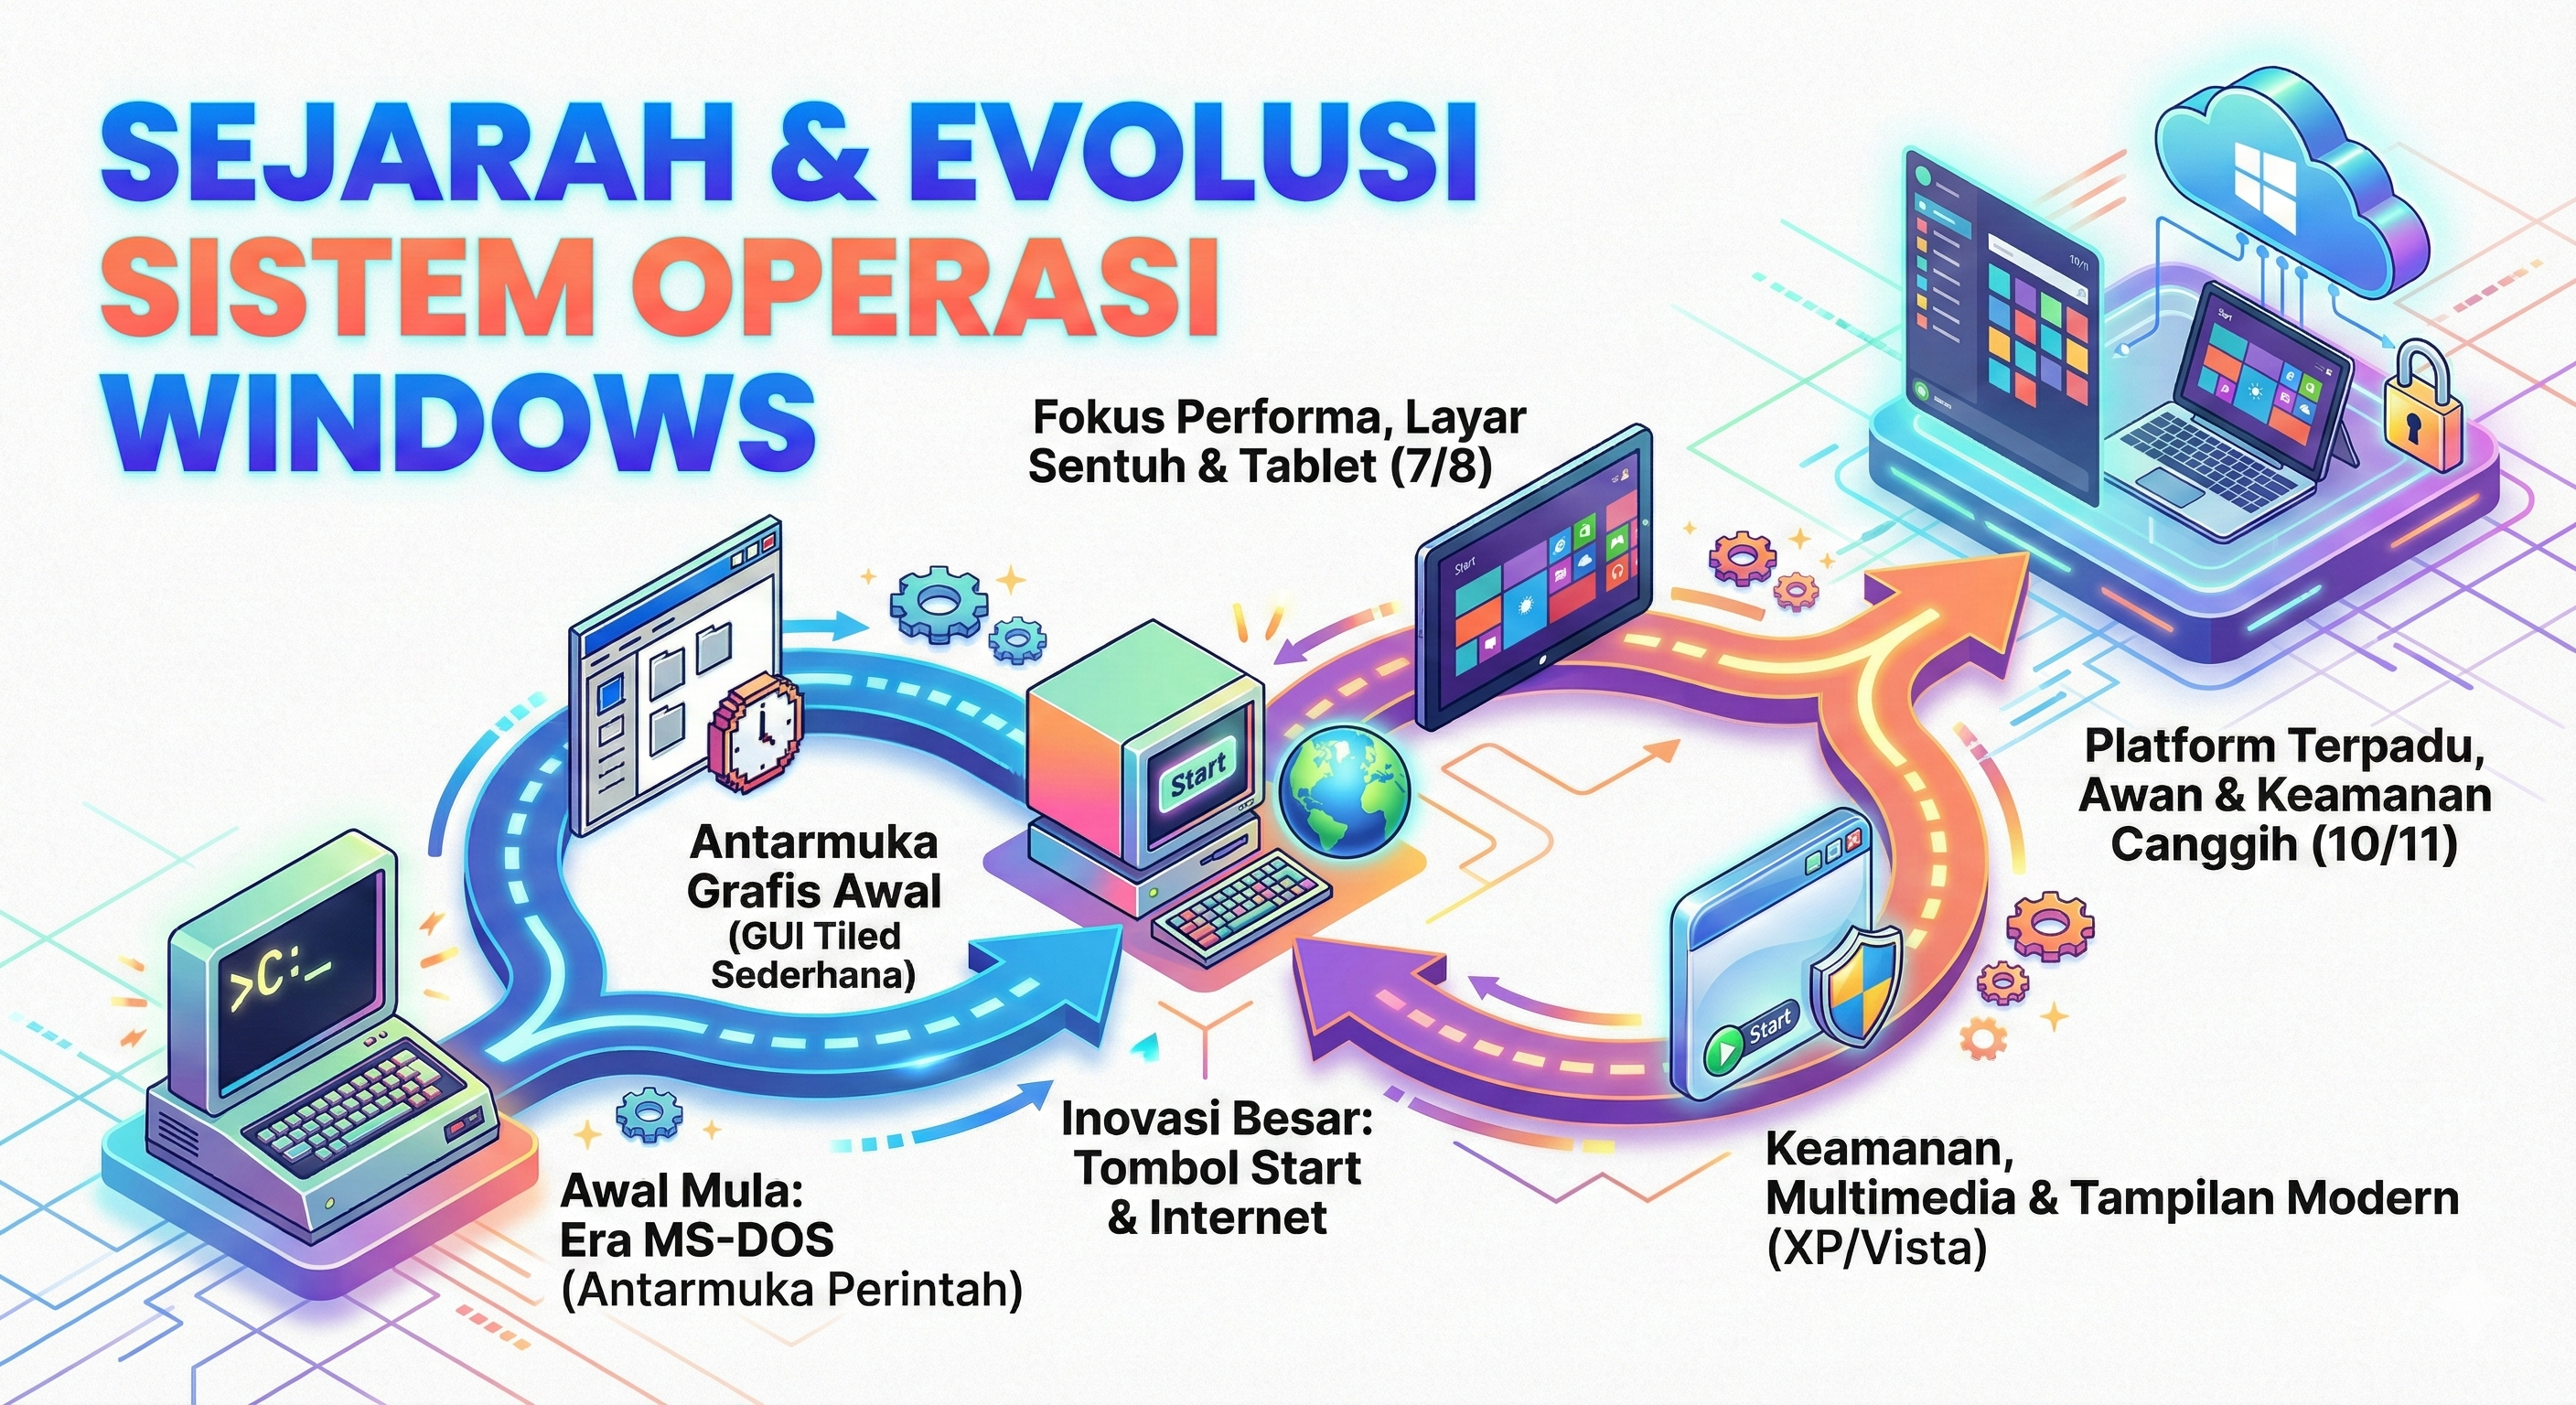
\includegraphics[width=0.93\paperwidth,keepaspectratio]{figures/1_winevo.png}
    \vfill
\end{frame}

%------------------------------------------------
%	CLASS ACTIVITY 2
%------------------------------------------------
\begin{frame}[t]
    \frametitle{Aktivitas Kelas: Evolusi Antarmuka (GUI)}
    \framesubtitle{Mengamati Transformasi Windows}

    \begin{block}{Tugas Pengamatan}
        Cari gambar tampilan desktop/start menu dari OS Windows berikut:
        \begin{center}
            \textbf{98 $\rightarrow$ 2000 $\rightarrow$ ME $\rightarrow$ XP $\rightarrow$ Vista $\rightarrow$ 7 $\rightarrow$ 10 $\rightarrow$ 11}
        \end{center}
    \end{block}
    
    \textbf{Diskusikan \& Beri Tanggapan:}
    \begin{itemize}
        \item Apa transformasi visual terbesarnya? (Misal: Flat vs 3D vs Glass/Aero).
        \item Adakah fitur yang "maju-mundur"? (Muncul, hilang, muncul lagi).
        \item \textit{Sharing}: Apa OS pertama yang Anda gunakan?
    \end{itemize}

    \vspace{0.2cm}
    \textit{Ketua Kelas / Asisten Dosen (Asdos) harap mencatat keaktifan partisipasi kelas melalui \textbf{lectura.id}.}
    
\end{frame}

\end{document}
